\documentclass{article}
\usepackage[utf8]{inputenc}
\usepackage{graphicx}

\title{Assignment 3}
\author{Tim Anema, Ivar de Bruin, Ilya Grishkov, \\Laura Pircalaboiu, Marc Otten}
\date{January 2020}

\begin{document}

\maketitle

\section{Assignment 3.1}
For this assignment we had to implement and document two (or more) design patterns. We decided to document the ones most heavily used by either server or client. For example, the client uses factories to handle creation of certain game objects, while the server relies on the strategy pattern to maintain its flexibility. 
\par Two of our most used patterns are the strategy pattern and the builder pattern. 

\subsection{The strategy pattern}
In this first section we will document the strategy pattern, which is heavily utilized on the server.

\subsubsection{Natural language description}
We use the strategy pattern on our server, in order to keep it
flexible. We use a considerable amount of interfaces to achieve this:
all components use interfaces to refer to other components, which means
we can change strategies during run-time. This way the server can adapt to
new technologies, without needing a rewrite.

\par For example: our server needs a database to function. A database needs to
provide two services: a user store and a score store. Those stores also need
to provide a predetermined set of services. From the server's viewpoint, it
does not matter what the actual database is, as long as it provides the
expected services. That's why the server depends on a set of interfaces
representing the services, and we provided an implementation based on a SQL
database. In theory, though, one could add another implementation based on
a NoSQL database and the server would happily use that too, as long as it
implements the required services.

\subsubsection{Class diagram}
Figure \ref{fig:strategy_dp} in the Appendix shows the class diagram of this design pattern in our case. A higher resolution can be found on our repository.

\subsubsection{Implementation}
The code for this design pattern can be found on our GitLab repository. More specifically in the server module, where the code for this design pattern is used in the Server class, where its required services (fields) are interfaces. More code on this design pattern can be found all throughout the server module.

\subsection{The builder pattern}
Besides the strategy pattern, we also use the builder pattern all throughout our code. For this assignment we decided to focus on a single class 'Score' in the shared module, but the pattern itself is used in all modules.

\subsubsection{Natural language description}
We use the library Lombok to reduce Java boilerplate, which also includes things like the builder pattern.
We normally annotate a class with @Builder, and Lombok will generate appropriate
bytecode at compile-time. For the sake of this exercise we also made a
'manual' builder for the Score class. We implemented this manual builder,
by creating an inner class, which contain builder functions. When all
properties are set, a build() call can be made, which instantiates the object.

\par We use the builder pattern, because some fields are optional and we want to
prevent creating a lot of constructors doing the exact same thing with small
variation. When a field is not optional, we enforce this by annotating said
field with @NonNull, which verifies our code at compile-time and adds checks
for enforcing this during run-time.

\subsubsection{Class diagram}
Figure \ref{fig:builder_dp} in the Appendix shows the class diagram of this design pattern in our case. A higher resolution can be found on our repository.

\subsubsection{Implementation}
The code for this design pattern can be found on our GitLab repository. In this assignment we used the Score class in the shared module, but this pattern can be found all throughout our repository, this includes all modules (shared, client and server). Please note that we normally use Lombok to use builders (@Builder or @SuperBuilder), so even though it might not seem like we use builders a lot, every annoted class uses this.

\section{Assignment 3.2}
\subsection{Motivation}
We decided to go for a Client-Server architecture because we thought it would make the most sense as the game lends itself to a client, who runs the actual game presented to the user, and a server, that stores the data about users and scores.
\subsection{Client}
\subsubsection{GameLogic}
This is the package that contains all the logic. It contains a number of packages containing the gameobjects (such as the table, balls, cue...), and their respective factories, as well as an abstract GameObject class.

\subsubsection{Games}
The Games package contains three classes that do most of the player-handling and rule-checking for the different kinds of games. We currently have an abstract game class, a 9-ball class and an 8-ball class.
\subsubsection{Requests}
The Requests package is where the connections to the server are actually sent. There is a class that sets up a Retrofit client to make the requests, and interfaces and classes for the requests we want to make (handling authentication and scoring). 
\subsubsection{Screens}
The Screens package is mostly GUI-related classes that set-up the screens that are actually shown to the user. They are connected to the classes in Requests because whenever a user pushes a button a request is made.
\subsubsection{Utils}
The Utils package contains some utilities such as a vector class and a class containing helpful constants. 
\subsection{Shared}
\subsubsection{Entity}
The Entity package contains classes that can be accessed both by the client and server. They are objects that can be serialized, so that the client and server both agree on how to represent, for example, the User object. 
The package is divided in auth and store.
\subsection{Server}
\subsubsection{Entity}
The Entity package provides interfaces for storing users and scores into the database. Those interfaces are implemented specifically for SQL, in the {\it impl} package. Things like connecting to the database and accessing it happen here.
\subsubsection{Http}
The Http package sets up endpoints on the server so that the client can talk to the server. Here the server sets up paths and sends responses, and the different endpoints are split into two packages: auth and score, where one takes care of the authentication and the other of leaderboard related requests.There is also a ping endpoint, which is useful for debug purposes.

\subsubsection{jwt}
This package takes care of the signing and verifying of authentication tokens, using JWT.
\subsubsection{storage}
This package takes care of the Database. It contains some Util classes to configure hibernate and some Entities to build instances to store in the DB.

\section{Appendix}
\begin{figure}
    \centering
    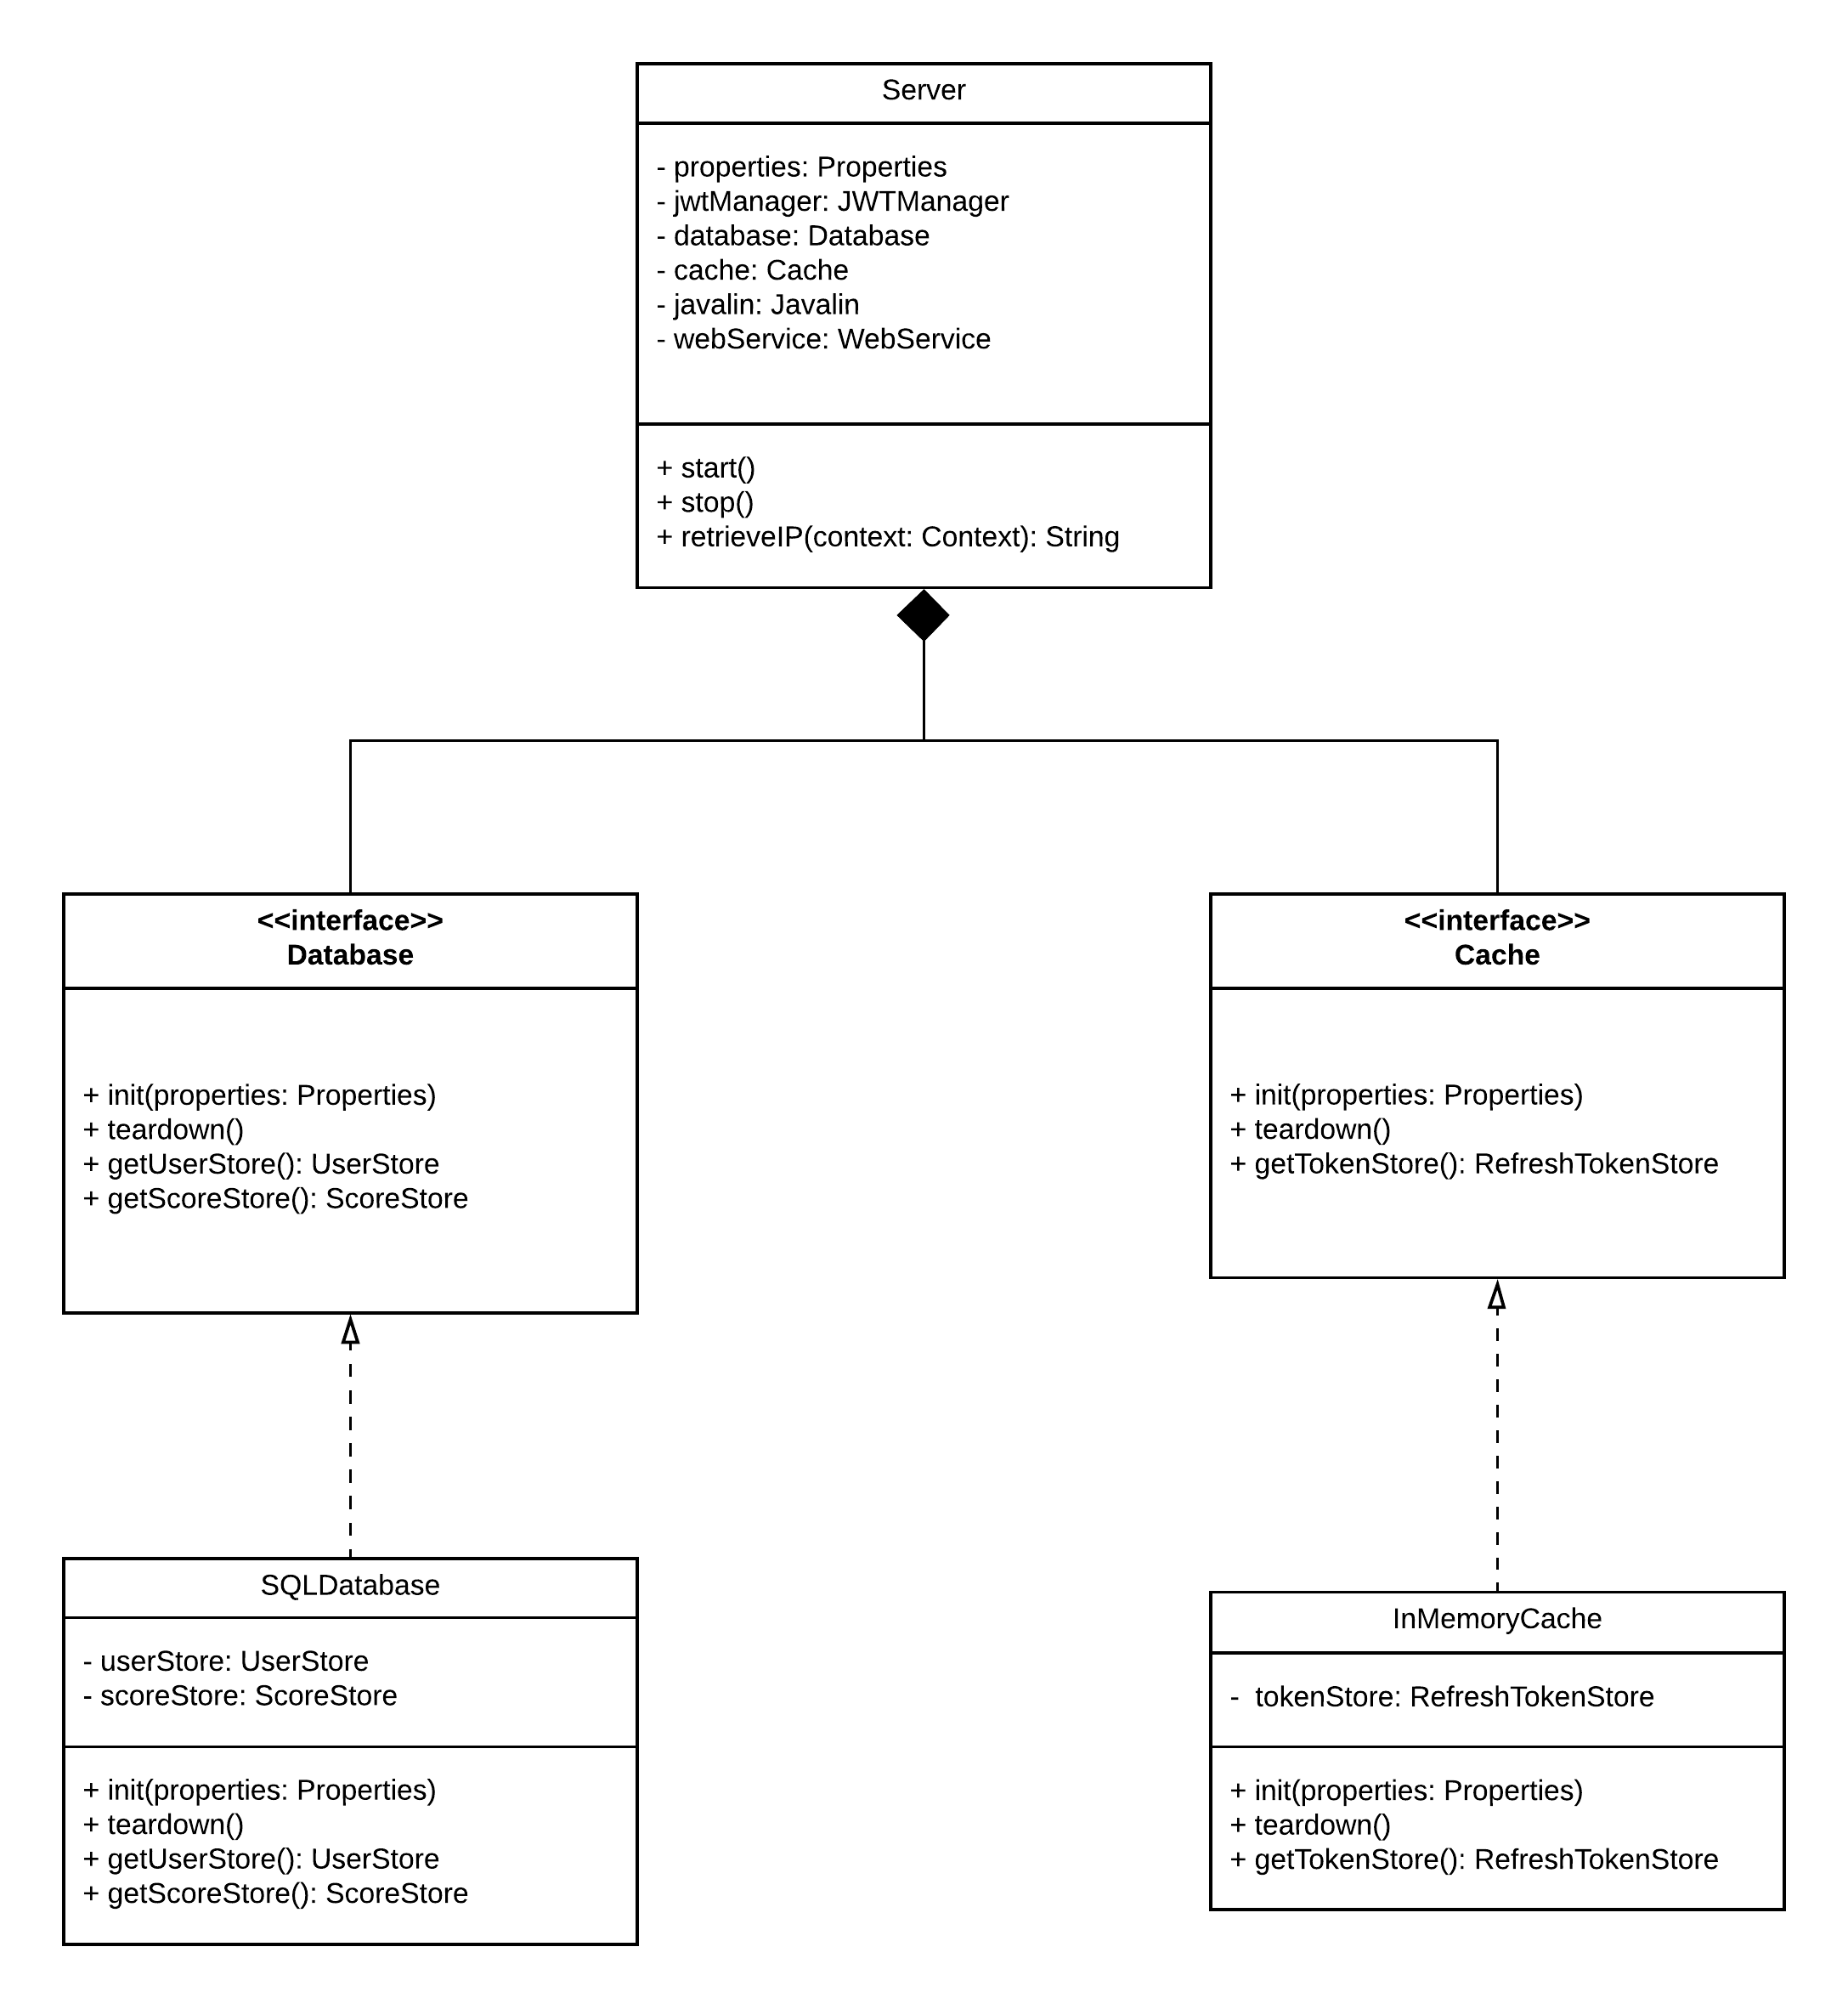
\includegraphics[width=\textwidth]{strategy_pattern.png}
    \caption{The class diagram for the strategy pattern}
    \label{fig:strategy_dp}
\end{figure}

\begin{figure}
    \centering
    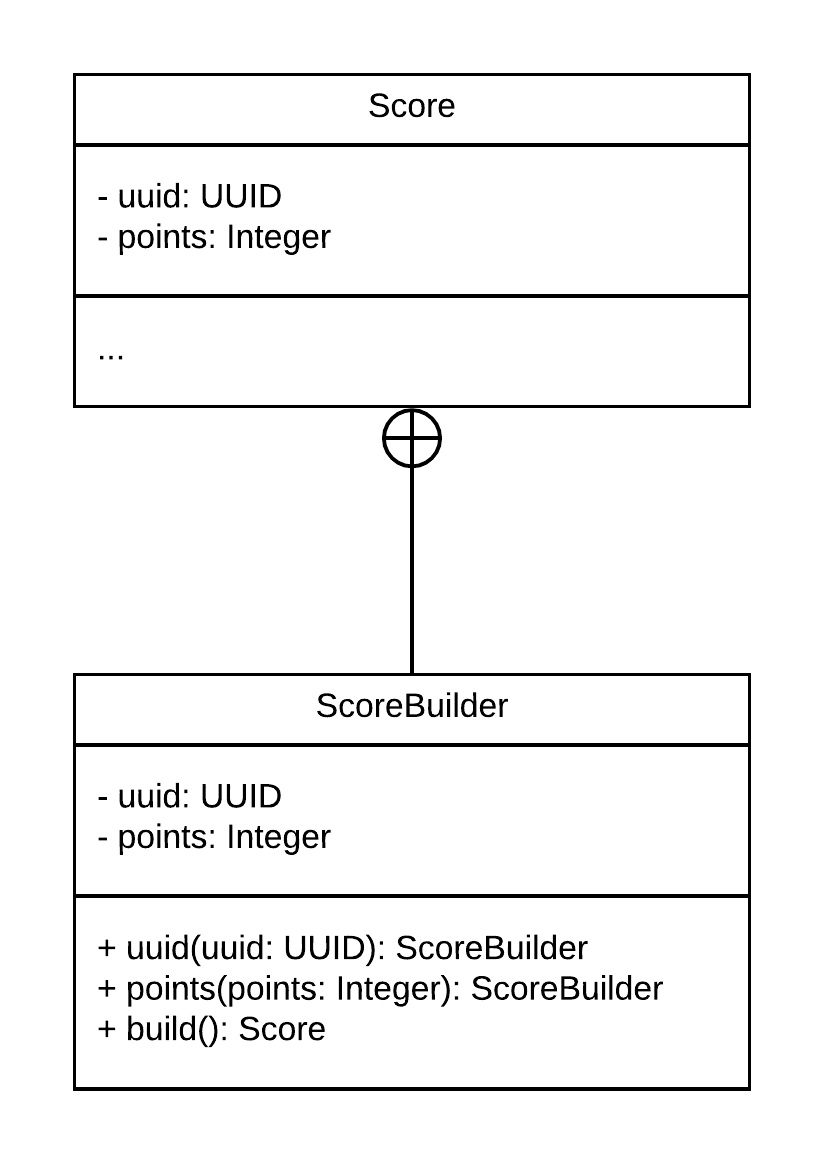
\includegraphics{builder_pattern.png}
    \caption{The class diagram for the builder pattern}
    \label{fig:builder_dp}
\end{figure}

\begin{figure}
    \centering
    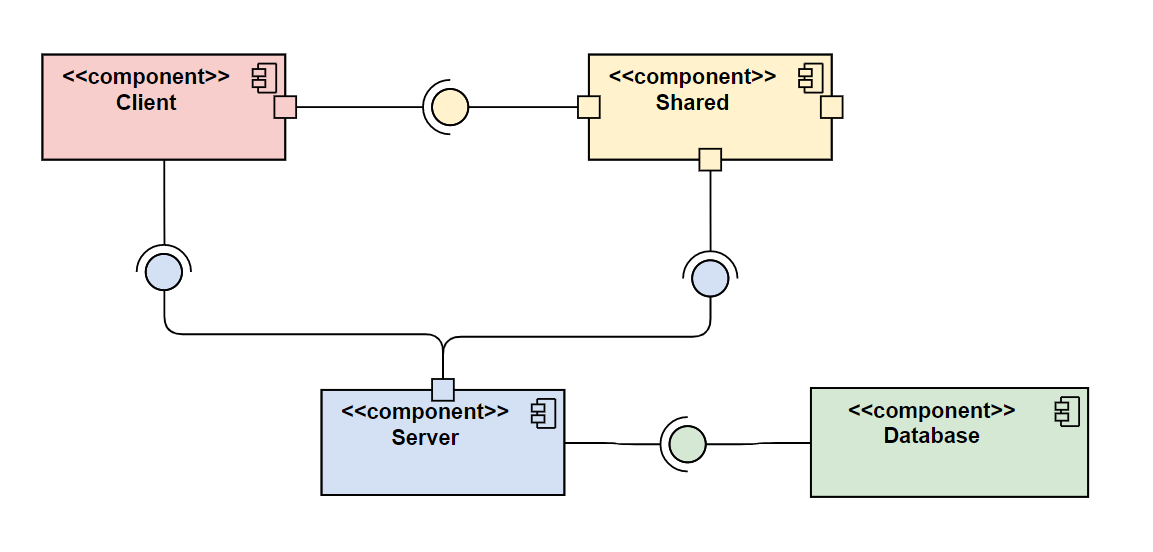
\includegraphics[scale = 0.5]{server_client.png}
    \caption{The architecture (component) diagram for the application}
    \label{fig:builder_dp}
\end{figure}
\end{document}
